\section{Introduction}

\begin{figure}[h!]
	\centering
	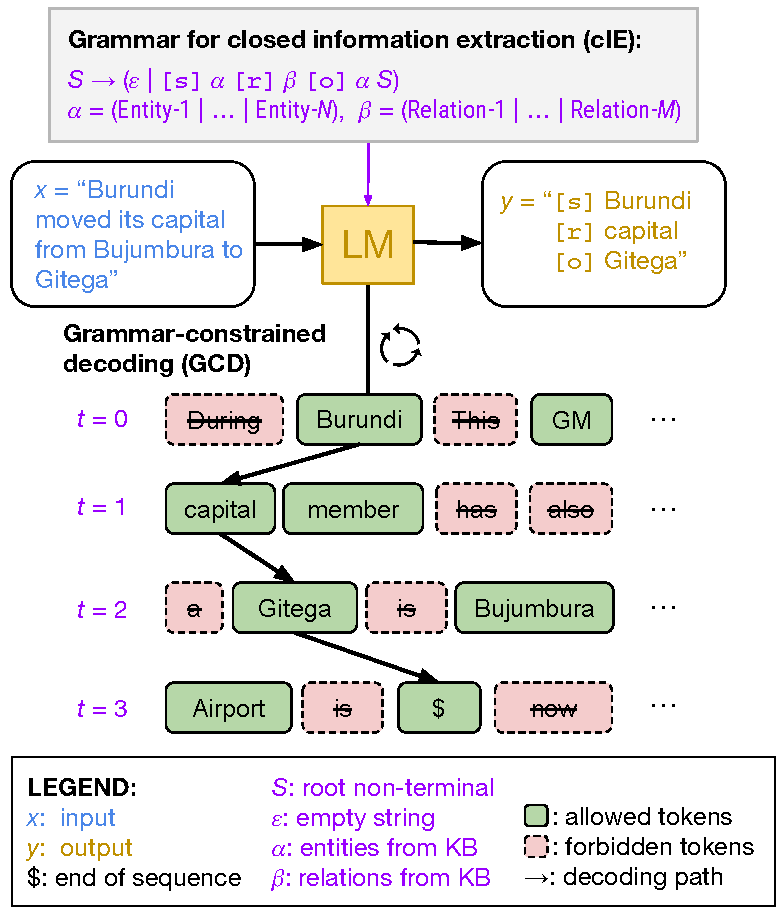
\includegraphics[width=0.9\linewidth]{img/intro_figure}
	\caption{\textbf{Grammar-constrained decoding (GCD),}
    applied to the task of closed information extraction, where the goal is to extract a list $y$ of subject--relation--object triplets from the input text $x$. Subjects and objects are constrained to be Wikidata entities, relations to be a Wikidata relation.
	During decoding, only valid token continuations compliant with the grammar are considered. For simplicity, we omit the special marker symbols \texttt{[s]}, \texttt{[r]}, and \texttt{[o]} in the schema of the generation process.}
	\label{fig:intro_figure}
\end{figure}

% \textbf{Motivation, problem}
Pretrained language models (LMs) have achieved impressive results across a range of tasks, such as machine translation, summarization, and dialogue generation~\cite{brown2020language, touvron2023llama}.
All of these models are pretrained on next-token prediction task, encouraging researchers to cast other NLP tasks in the same autoregressive generation framework.
By framing tasks as autoregressive generation, pretrained language models can be finetuned for specific tasks with minimal modifications to the training process while still benefiting from the advantages of pretraining.
More recently, the scaling of language models to larger sizes has introduced notable in-context learning capabilities \cite{brown2020language, Radford2019LanguageMA, schick-schutze-2021-exploiting}, such that large language models (LLMs) can quickly and effectively adapt to new tasks even without finetuning, when shown only few demonstrations as part of their context.

% Building upon these successes, researchers have formulated most Natural Language Processing (NLP) tasks as autoregressive generation problems, leveraging the specific strengths of LMs.


Certain important tasks, however, such as closed information extraction (cIE), entity disambiguation (ED), or constituency parsing (CP), require the output to follow a predefined format and adhere to a restricted vocabulary (entities, relations, senses, dependency labels, \etc).
Whereas LMs excel at generating free-form text, they are not specifically designed for structured prediction tasks where only a small subset of the output space is valid.
Consequently, structured prediction tasks present unique challenges because constrained output spaces demand both structural coherence and compliance with a predefined vocabulary.
For instance, \citet{josifoski2023exploiting} have demonstrated that few-shot-prompted large language models such as GPT-3.5 struggle with tasks such as cIE. This difficulty is primarily due to the extensive output vocabulary, which includes 2.7 million Wikidata entity names and approximately 1,000 Wikidata relation names, which is too vast to be conveyed with just a few demonstration examples.

One way forward is to finetune LMs for specific tasks, which involves linearizing the desired output format into a string format, thus enabling training through standard next-token prediction.
For instance, \citet{decao2021autoregressive} and \citet{josifoski-etal-2022-genie} successfully applied this technique to ED and cIE, respectively.
However, this approach has limitations: it necessitates an expensive finetuning pipeline for each new task, which lacks flexibility and requires bespoke training data.
Orthogonally, constrained decoding~\cite{tromble-eisner-2006-fast} is a technique that can be used to enforce constraints on the output space of an autoregressive language model during inference.
Constrained decoding has been used in semantic role labeling~\cite{deutsch-etal-2019-general}, constituency parsing~\cite{deutsch-etal-2019-general},  code generation~\cite{scholak-etal-2021-picard}, and entity disambiguation~\cite{decao2021autoregressive}.
The constraints have been expressed in the form of finite-state automata~\cite{deutsch-etal-2019-general} or trie-based data structures for fast lookup~\cite{decao2021autoregressive}.


In this work, we show that, for a much wider range of NLP tasks, the respective output space can be described with a formal grammar, giving rise to a unified framework for structured NLP tasks.
Given an appropriately defined grammar, we use an {incremental parser} to play the role of a completion engine, which determines the set of valid next tokens given the current {prefix}.
We integrate this completion engine with a pretrained language model to iteratively generate sequences that are \textit{valid} according to the grammar and \textit{plausible} according to the LM (\cf\ \Figref{fig:intro_figure}).
From a practical perspective, the \textit{grammar-constrained decoding} (GCD) framework allows researchers to focus on writing the grammar while ignoring the implementation details of the constrained decoding process.
This is in contrast to previous work, where the constraints were expressed in the form of finite-state automata or trie-based data structures, which require a significant engineering effort to implement.
%We envision that GCD will play a similar role as RegEX, where the user can specify the desired output structure in a declarative way, and the generation from LMs will be valid sequences.
We envision GCD to be as simple to use as regular expressions, in the sense that the user can specify a desired output structure in a declarative way, and the LM-generated sequences will be guaranteed to be valid.
With the introduction of \textit{input-dependent grammars,} the scope of tasks that can be tackled with GCD can be further extended to tasks such as entity disambiguation and entity linking, where the output space is not fixed but depends on the input.
We show that, by combining GCD with powerful LLMs, we achieve remarkable improvements with few-shot learning, even rivaling the performance of finetuned task-specific models.
This is particularly exciting because it shows that LMs can be used to solve a much wider range of structured tasks than before, without the need for finetuning.



Our contributions can be summarized as follows:
\begin{enumerate}[itemsep=0pt, parsep=0pt]
\item We demonstrate that the output spaces of many structured NLP tasks can be formulated as formal languages, thus converting the tasks into grammar-constrained decoding problems. This formulation provides a unified framework to tackle structured NLP tasks.
\item We introduce input-dependent grammars, which extend the set of tasks that can be tackled with GCD.  We show that this can be useful, among others, for tasks such as ED and CP.
\item Through empirical experiments, we demonstrate the effectiveness of GCD on three structured NLP tasks: cIE, ED, and CP.  We show that our method can achieve competitive results on cIE and ED without any finetuning.
\end{enumerate}

%Our findings indicate that the integration of grammar-based constraints during decoding is a promising approach for making LMs reliably produce structured outputs. This research paves the way for further advancements in making LMs more proficient in producing more accurate and controlled outputs.

\begin{figure}[t]
%\vspace{-20pt} % Reduces space above the figure
	\centering
	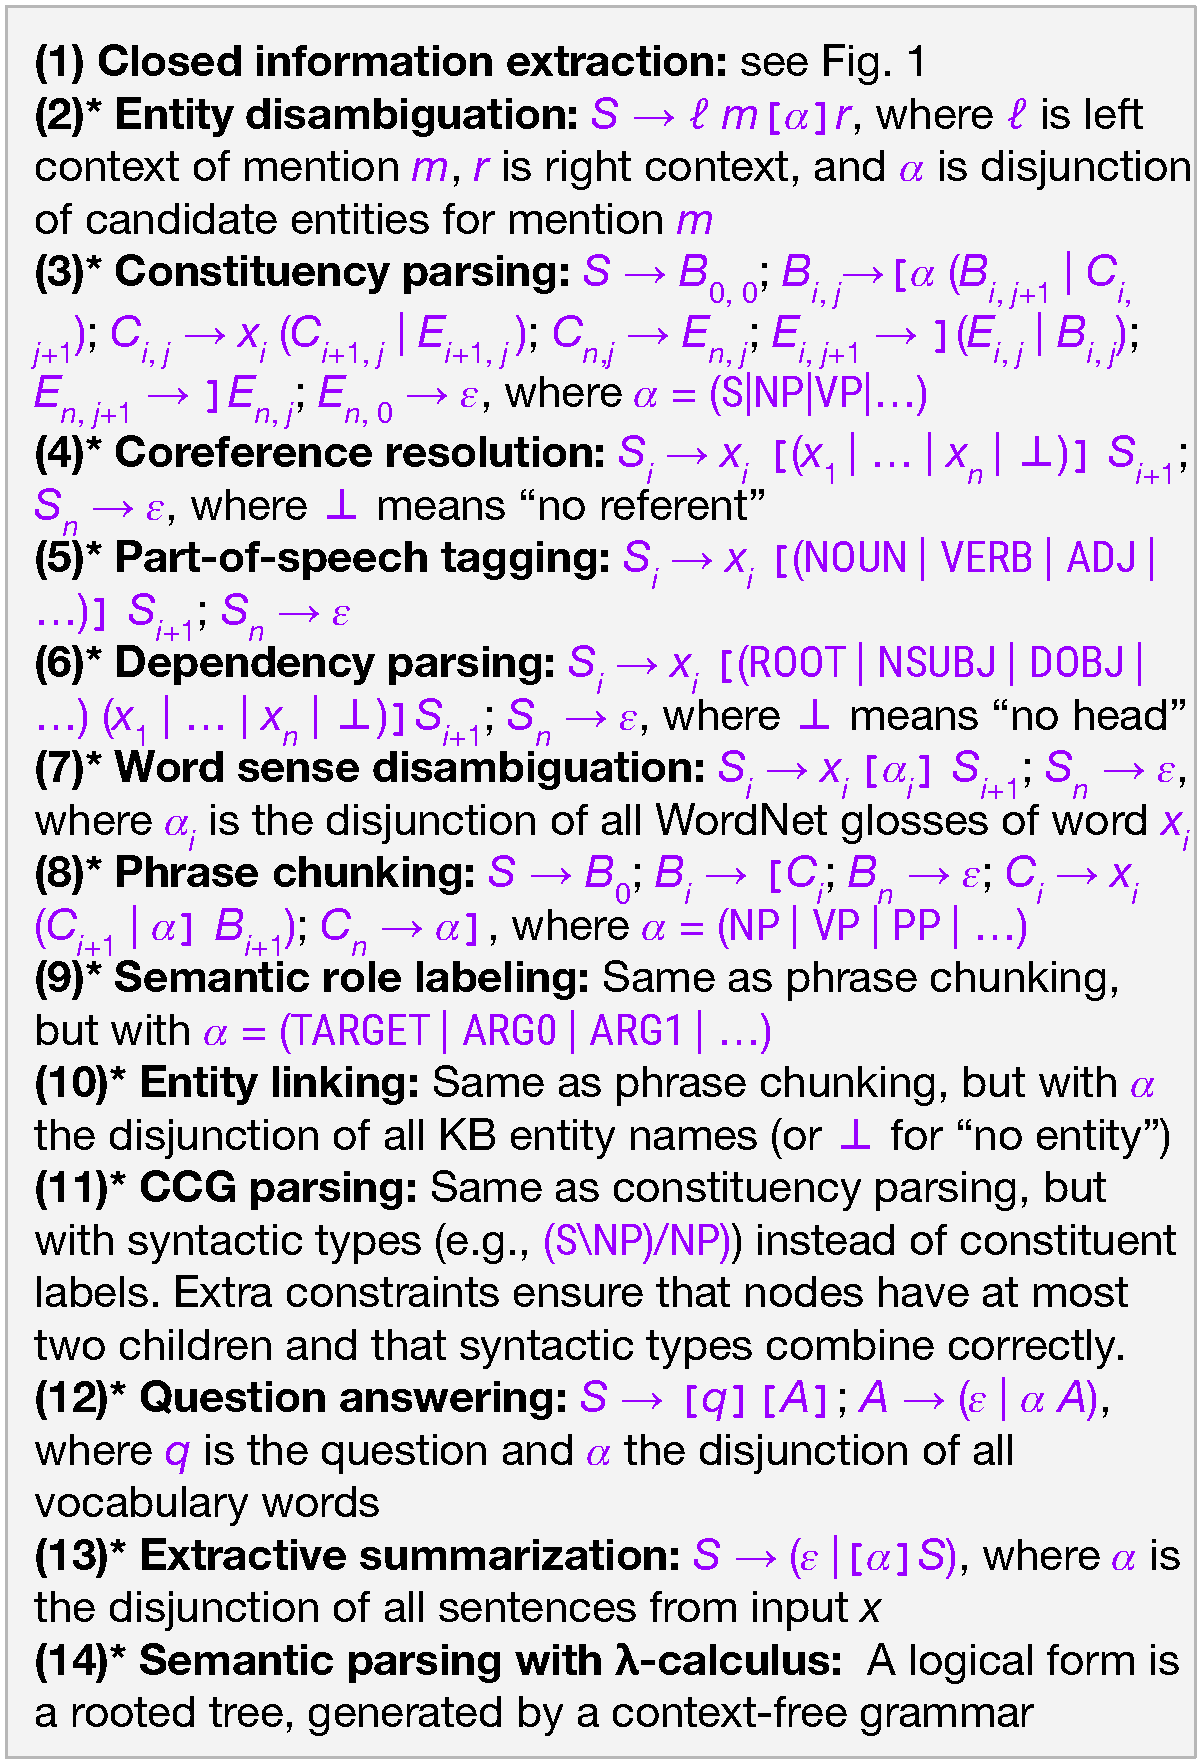
\includegraphics[width=1.0\linewidth]{img/Grammars-showcase}
	\caption{\textbf{Formal grammars for 14 structured NLP tasks,}
	highlighting the general applicability of grammar-constrained decoding.
 All 14 grammars are context-free (mostly regular).
	* marks input-dependent grammars. 
 Inputs $x=\langle x_0, \dots, x_{n-1} \rangle$ are sequences of lexical units (\eg, words); $0 \leq i \leq n-1$; single capital letters are non-terminal symbols; $S$ or $S_0$ is the start symbol; $\varepsilon$ is the empty string; \texttt{[} and \texttt{]} are special terminal symbols.}
	\label{fig:grammars_showcase_more}
%\vspace{-20pt} % Reduces space below the figure
\end{figure}